%
% Complete documentation on the extended LaTeX markup used for Insight
% documentation is available in ``Documenting Insight'', which is part
% of the standard documentation for Insight.  It may be found online
% at:
%
%     http://www.itk.org/

\documentclass{InsightArticle}

\usepackage[dvips]{graphicx}
%\usepackage{listing}						
\usepackage{listings}	
\usepackage{wrapfig}
\usepackage{amssymb,amsmath}
\usepackage{multirow,booktabs,array}
\usepackage{listings}
\usepackage{color}
				
%%%%%%%%%%%%%%%%%%%%%%%%%%%%%%%%%%%%%%%%%%%%%%%%%%%%%%%%%%%%%%%%%%
%
%  hyperref should be the last package to be loaded.
%
%%%%%%%%%%%%%%%%%%%%%%%%%%%%%%%%%%%%%%%%%%%%%%%%%%%%%%%%%%%%%%%%%%
\usepackage[
bookmarks,
bookmarksopen,
backref,
colorlinks,linkcolor={blue},citecolor={blue},urlcolor={blue},
]{hyperref}




\graphicspath{{./Figures/}}
\newcommand{\fv}{\mbox{\boldmath $f$}}
\newcommand{\Iv}{\mbox{\boldmath $I$}}
\newcommand{\xv}{\mbox{\boldmath $x$}}
\newcommand{\velocity}{\mbox{\boldmath $v$}}
\newcommand{\velocityinv}{\mbox{\boldmath $v$}^{-1}}
\newcommand{\Velocityinv}{\mbox{\boldmath $V$}^{-1}}
\newcommand{\Velocity}{\mbox{\boldmath $V$}}
\newcommand{\welocity}{\mbox{\boldmath $w$}}
\newcommand{\spatialimagegradient}{\mbox{\boldmath $I$}\mbox{$_{x}$}}
\newcommand{\perpspatialimagegradient}{\mbox{\boldmath $I$}\mbox{$^{\perp}_{x}$}}
\newcommand{\temporalimagederivative}{\mbox{$I_t$}}
\newcommand{\finitestrain}{\mbox{\boldmath $\varepsilon^{\ast}$}}
\newcommand{\smallstrain}{\mbox{\boldmath $\varepsilon$}}
\newcommand{\dispgradient}{{\bf \nabla \displace}}
\newcommand{\displace}{{\bf u}} 
\newcommand{\Id}{\text{\bf Id}}
\newcommand{\ode}{{\em O.D.E.}}
\newcommand{\odes}{{\em O.D.E.}s}
\newcommand{\G}{\mathcal{G}}
\newcommand{\J}{\mathcal{J}}
\newcommand{\phiinv}{\phi^{-1}}
\newcommand{\psiinv}{\psi^{-1}}
\newcommand{\dM}{DM}
\newcommand{\DM}{Diffeomorphometry}
\newcommand{\diff}{diffeomorphism}
\newcommand{\Diff}{Diffeomorphism}
\newcommand{\orbit}{\mathcal{O}}
\newcommand{\avg}{\mathcal{A}}
\newcommand{\avgn}{\mathcal{A}_n}
\newcommand{\avgna}{\mathcal{A}^a_{n}}
\newcommand{\nset}{\{ J_i \}_n}
\newcommand{\bari}{\bar{I}}
\newcommand{\bart}{\bar{t}}
\newcommand{\jac}{\mathcal{J}}
\newcommand{\pert}{\mbox{\boldmath $w$}}
\newcommand{\barpert}{\bar{\mbox{\boldmath $w$}}}
\newcommand{\half}{0.5}

\newcommand{\X}{{\bf X}}
\newcommand{\x}{{\bf x}}
\newcommand{\Z}{{\bf Z}}
\newcommand{\z}{{\bf z}}
\newcommand{\p}{{\bf p}}
\newcommand{\Y}{{\bf Y}}
\newcommand{\y}{{\bf y}}
\newcommand{\disp}{{\bf u}}
\newcommand{\ytild}{\tilde{{\bf y}}}
\newcommand{\q}{{\bf q}}
\newcommand{\surf}{\mathcal{S}}
\newcommand{\phij}{\phi_{ij}}
\newcommand{\aphij}{\bar{\phi}_{j}}
\newcommand{\apsij}{\bar{\psi}_{j}}
\newcommand{\aphi}{\bar{\phi}}
\newcommand{\aphiinv}{\bar{\phi}^{-1}}

\newcommand{\domain}{\Omega}
\newcommand{\meanshape}{\bf \bar{x}}
\newcommand{\g}{\mbox{\boldmath $g$}}
\newcommand{\h}{\mbox{\boldmath $h$}}
\newcommand{\yv}{\mbox{\boldmath $y$}}

\newcommand{\group}{Diff}


\newcommand{\evol}{{E_{\text{Vol}}}}
\newcommand{\epair}{{E_{\text{Pair}}}}
\newcommand{\esec}{{E_{S}}}
\newcommand{\inv}{^{-1}}
\newcommand{\vinit}{ \velocity^0_{ij}(\x,\tau=0) }
\newcommand{\avinit}{ \bar{\velocity}^0_{j}(\x,t) }
\newcommand{\avinitz}{ \bar{\velocity}^0_{j}(\x,t_a) }
\newcommand{\gz}{\nabla_{\z}}


 
\definecolor{dkgreen}{rgb}{0,0.6,0}
\definecolor{gray}{rgb}{0.5,0.5,0.5}
\definecolor{mauve}{rgb}{0.58,0,0.82}

\lstset{ %
  language=bash,                % the language of the code
  basicstyle=\footnotesize,           % the size of the fonts that are used for the code
  numbers=left,                   % where to put the line-numbers
  numberstyle=\tiny\color{gray},  % the style that is used for the line-numbers
  stepnumber=2,                   % the step between two line-numbers. If it's 1, each line 
                                  % will be numbered
  numbersep=5pt,                  % how far the line-numbers are from the code
  backgroundcolor=\color{white},      % choose the background color. You must add \usepackage{color}
  showspaces=false,               % show spaces adding particular underscores
  showstringspaces=false,         % underline spaces within strings
  showtabs=false,                 % show tabs within strings adding particular underscores
  frame=single,                   % adds a frame around the code
  rulecolor=\color{black},        % if not set, the frame-color may be changed on line-breaks within not-black text (e.g. commens (green here))
  tabsize=2,                      % sets default tabsize to 2 spaces
  captionpos=b,                   % sets the caption-position to bottom
  breaklines=true,                % sets automatic line breaking
  breakatwhitespace=true,        % sets if automatic breaks should only happen at whitespace
  prebreak=\textbackslash, breakindent=7pt,
  title=\lstname,                   % show the filename of files included with \lstinputlisting;
                                  % also try caption instead of title
  keywordstyle=\color{blue},          % keyword style
  commentstyle=\color{dkgreen},       % comment style
  stringstyle=\color{mauve},         % string literal style
  escapeinside={\%*}{*)},            % if you want to add a comment within your code
  morekeywords={*,...}               % if you want to add more keywords to the set
}


%  This is a template for Papers to the Insight Journal. 
%  It is comparable to a technical report format.

% The title should be descriptive enough for people to be able to find
% the relevant document. 
\title{The PipeDream Neuroimaging Pipeline for Cross-Sectional and Longitudinal Studies of Cortex and Connectivity}

% 
% NOTE: This is the last number of the "handle" URL that 
% The Insight Journal assigns to your paper as part of the
% submission process. Please replace the number "1338" with
% the actual handle number that you get assigned.
%
%\newcommand{\IJhandlerIDnumber}{}

% Increment the release number whenever significant changes are made.
% The author and/or editor can define 'significant' however they like.
\release{1.00}

% At minimum, give your name and an email address.  You can include a
% snail-mail address if you like.
\author{P.Cook, B. Avants, N. Tustison, Y. Zheng, J. Duda, J. Gee}
\authoraddress{Penn Image Computing And Science Laboratory\\
University of Pennsylvania}

\begin{document}

%
% Add hyperlink to the web location and license of the paper.
% The argument of this command is the handler identifier given
% by the Insight Journal to this paper.
% 
%\IJhandlefooter{\IJhandlerIDnumber}


\ifpdf
\else
   %
   % Commands for including Graphics when using latex
   % 
   \DeclareGraphicsExtensions{.eps,.jpg,.gif,.tiff,.bmp,.png}
   \DeclareGraphicsRule{.jpg}{eps}{.jpg.bb}{`convert #1 eps:-}
   \DeclareGraphicsRule{.gif}{eps}{.gif.bb}{`convert #1 eps:-}
   \DeclareGraphicsRule{.tiff}{eps}{.tiff.bb}{`convert #1 eps:-}
   \DeclareGraphicsRule{.bmp}{eps}{.bmp.bb}{`convert #1 eps:-}
   \DeclareGraphicsRule{.png}{eps}{.png.bb}{`convert #1 eps:-}
\fi


\maketitle


\ifhtml
\chapter*{Front Matter\label{front}}
\fi



% The abstract should be a paragraph or two long, and describe the
% scope of the document.
\begin{abstract}
\noindent PipeDream uses open-source software to help neuroimaging researchers perform advanced processing with state-of-the-art techniques.  PipeDream performs data reconstruction, data organization, advanced brain extraction, bias correction, three tissue classification and cortical thickness estimation.  Diffusion tensor processing, unbiased longitudinal analysis and cortical parcellation are available as advanced options.  PipeDream relies on prior knowledge encoded in an optimal template.  PipeDream also helps one review the processing and perform quality assurance.  The tool documents our current ``best practice'', implementable with free software, for MRI-based studies of the brain.
\end{abstract}

%\IJhandlenote{\IJhandlerIDnumber}

\tableofcontents
\newpage
\section*{Introduction}
Additional information is available online -- see 
\href{https://sourceforge.net/projects/neuropipedream/}\\{PipeDream
  Homepage :
  https://sourceforge.net/projects/neuropipedream/} 

Pipedream requires the ANTS package and dcm2nii from mricron as well as Camino if you are doing DTI processing.  Google ``ANTS picsl'' for ANTS.  These programs may be installed already so please check before installing.

The pipedream neuroimaging pipeline has five stages: 
\begin{enumerate}
\item Organize data.
\item Construct a template.  
\item Run the brain processing pipeline.  
\item Check results. 
\item Perform statistical analyses.  
\end{enumerate}

We cover each step in turn, briefly, here. 


\footnote{This document is a work in progress. Please check for updates with each release.}

\section{Data Organization and study design}

Correct data organization should begin at the study design phase. Subject identifiers should uniquely identify a subject and should not contain protected health information. Time points should be identified as specifically as possible, preferably with scan dates rather than symbolic names. If a study involves multiple sources of information, for example demographic information and imaging, the data organization should be planned ahead of time to facilitate interoperability.

Choosing subject and scan identifiers intelligently is important for facilitating scripting, for ensuring data integrity, and for integrating imaging with other information, for example from a database. A common error is to choose conventions that are easily navigable by humans, but not by computers. A human can easily interpret $1/1/01$, $1/1/2001$, $01/01/2001$, ``1 Jan 2001", ``January 1st 2001", as the same information, but a computer will think these are all different unless it has been specially trained to interpret dates. It is much better to rely on literal equivalence, for dates we recommend use of the ``YYYYMMDD'' date format, which allows computers to naturally sort dates correctly. This makes it easier to do things like pick the first scan for a given subject.

An example of a good naming convention is to use a fixed-width, five-digit number to uniquely identify each subject both in an online database and in the imaging repository, with a scan date in the format YYYYMMDD. For example, if subject 42001 is scanned on July 1st 2010, then his data would be found in the directory $42001/20100701/$. Now we can easily see when each visit was and compute how much time elapsed between them, which is important for longitudinal studies. 

Subject identifiers should be alphanumeric and not include special characters that may cause problems for scripts. Alphanumeric includes all letters and numbers, plus the underscore character \_. Other characters have special meaning in various software packages and may cause problems. 

\section{Tools for processing DICOM data}

The tools in this section will allow you to organize your DICOM data in Pipedream format and convert it to NIfTI for postprocessing.

The PipeDream format is $basedir/subject/timepoint/modality$.  The ``modality''  name must uniquely identify each scan that is acquired in a particular visit. Sometimes there may be multiple image series for a particular modality, for example if an imaging series is repeated in order to boost signal to noise. In this case, scans should be distinguished with a leading number, for example 0002\_t1\_mpr\_AX\_MPRAGE, 0003\_t1\_mpr\_AX\_MPRAGE. Scan names should not be a substring of another, eg if you have ``t1\_mpr\_AX\_MPRAGE'', you should not have ``AX\_MPRAGE'' in the same directory.

Scan names and directories should be alphanumeric. Spaces and other special characters will cause problems.

If your data is already organized this way, it is ready for Pipedream. Otherwise, you may wish to run dicom2series.
 

\subsection{dicom2series}

The dicom2series command is designed to organize dicom files into a Pipedream compatible format. The input data must be separated by subject, but need not be separated by date or modality. 
\begin{verbatim}
  dicom2series/dicom2series.sh <output_dir> <rename_files> <dicom_file1> ... <dicomfileN>
\end{verbatim}
Where output\_dir is the output directory, rename\_files is a flag set to 1 to rename files according to their header information, and 0 to preserve original file names. The input files can contain both dicom and non-dicom files (the latter will not be copied to the output directory), but must contain only files from a single subject. 

The data will be sorted into pipedream format. The output directory name should be the unique subject identifier, dicom2series will organize scans according to subject/timepoint/modality. The timepoint is the acquisition date. The ``modality'' is the series number and protocol name. 

Spaces and other metacharacters that are present in protocol names will be removed in the output.

The program may fail if your dicom files are strange, for example if they are missing series numbers. If you have a very large number of dicom files, or you have badly formatted data (eg, with spaces in the file names), the command line above may fail, but you can get around this with \textbf{xargs}. For example,
\begin{verbatim}
  find ./data/subject -type f -print0 | xargs -0 dicom2series.sh subjectsDICOM/subject 0
\end{verbatim}
will find all files inside $data/subject$ and pipe them to dicom2series in batches. 


\subsection{dicom2t1}

Once all subjects are organized in Pipedream format, the next step is to convert the DICOM T1 scans to NiFTI format. We recommend separating the DICOM and NIfTI base directories and making your DICOM data read-only.

This can be done in parallel or in series, depending on the number of subjects. The call is
\begin{lstlisting}
  dicom2t1/dicom2t1_batch.sh <queue_type> <subject_list> <protocol_list> <data_dir> <output_dir> blah blah blah blah 
\end{lstlisting}
Set queue type to ``sge'', ``voxbo'' to submit jobs to a cluster or ``none'' to run on the local machine. The subject list
is a newline separated list of subjects, such as you would get by typing
\begin{verbatim}
  ls subjectsDICOM > subjects.txt
\end{verbatim}
assuming you have not put other files or directories into subjectsDICOM.

The protocol list is a list of structural imaging protocols, typically this will contain only one line but sometimes
you may have more, for example for multi-site studies. The format is
\begin{verbatim}
  protocolName    shortName
\end{verbatim}
where the protocolName identifies the scan directory, and shortName is a string you want included in the output. For example,
\begin{verbatim}
  t1_mpr_AX_MPRAGE    mprage
\end{verbatim}
produces output files ending in ``mprage\_t1.nii.gz''. 

The next argument is simply subjectsDICOM/ where you have placed your organized DICOM files for each subject. Lastly, specify
an output directory. We recommend placing the output outside the directory structure where your original DICOM data reside.

The output from dicom2t1 is 
\begin{verbatim}
  output_dir/subject/timepoint/Anatomy/subject_timepoint_shortName_t1.nii.gz
\end{verbatim}
where the subject ID and the timepoint are taken from the DICOM directory, and shortName comes from the protocol file.


\subsection{dicom2dt}

Converting the DT is a bit more involved than the T1. The dicom2dt program not only converts to NIfTI, but also extracts
gradient directions, does distortion correction, and computes the diffusion tensor. You call the program in a similar way
\begin{verbatim}
  dicom2dt/dicom2dt_batch.sh <queue_type> <subject_list> <protocol_list> <data_dir> \
                              <output_dir>
\end{verbatim}
The files are defined the same way, except that the protocol file may point to a list of b-values and gradient vectors in FSL format.
Most users will not need to use this feature, and will just list protocol names as with T1. For example:

\begin{verbatim}
  DTI_30dir_noDiCo_vox2_1000    30dirdt
  DTI_12dir                     12dirdt        hup12dir.bval    hup12dir.bvec
\end{verbatim}

For the 12-direction protocols, dicom2dt will use the bval and bvec files to figure out the gradient directions 
and b-values in the data. These files are stored in FSL format, which is what is produced by dcm2nii. For ``30dirdt'' data, 
dicom2dt will figure out the b-values and gradients automatically. This option exists because dcm2nii does not get the gradient 
directions correctly for some data.

It's common to acquire repeat acquisitions of DWI images in the same scanning session. If this happens, then multiple folders
with the same protocol name will appear in the subject's dicom directory and dicom2dt will combine these automatically.

Motion and distortion correction is done with ANTS by computing affine registration of each DWI to the mean b=0 image. 
DT reconstruction is done using Camino's ``wdtfit'' program, more information can be found on the Camino website.
Brain extraction is performed using Atropos segmentation and some morphological operations.

Dicom2dt produces several outputs. All output is prefixed by ``subject\_timepoint\_protocol\_''.

\begin{table}[htdp]
\caption{default}
\begin{center}
\begin{tabular}{|c|c|}
\hline
\textbf{Output} & \textbf{Description} \\ \hline
allscans.scheme & The scheme file for the complete acquisition, including repeats if any. \\ \hline
averagedwi.nii.gz & The average of all images with $b > 0$. \\ \hline
brainmask.nii.gz & The brain / background binary mask, computed by segmenting the average DWI. \\ \hline
dt.nii.gz         & The diffusion tensors in NIfTI format. \\ \hline
dwi               & Directory containing corrected raw dwi images \\ \hline
exitcode.nii.gz   & Contains brain / background mask and flags for bad data. \\ \hline
lns0.nii.gz       & Reconstructed estimate of the log of the b=0 signal. \\ \hline
sigmaSq.nii.gz    & Estimate of the noise variance in each voxel \\ \hline
\end{tabular}
\end{center}
\label{dicom2dtout}
\caption{Output of dicom2dt}
\end{table}%


\section{Construct a Template}
Pipedream requires that you have a template---preferably constructed
from a dataset similar to your current study---with a number of
companion images that contain anatomical labels.  The minimum set of
priors include: a brain or cerebrum mask, a cerebrospinal fluid
probability map, a gray matter probability map and white matter
probability map.

If you do not have a template already available---or would like a local/optimal 
template---then you can build one from your data by following these steps:
\begin{enumerate}
\item Create a template directory where you can write a bunch of data.
\item Link your anatomical (T1-MRI) images into the directory, using ``ln -s'' in unix/linux/osx.
\item Call the ANTS command AverageImages to get an initial template
  or copy one of your subjects to a file called DIFFtemplate.nii.gz
  .... Make sure you don't copy a file called image.nii to a nii.gz
  file-type.  Either way, you will get an unbiased template out of this process.  
\item Call the ANTS script :   sh buildtemplateparallel.sh in this directory.  
  An example call is here: 
\begin{verbatim}
  sh buildtemplateparallel.sh -d 3 -o DIFF -c 2 -j 2 -z DIFFtemplate.nii.gz  *T1.nii.gz 
\end{verbatim}
  In this example, we assume you have images of the type   Sub001T1.nii.gz .
  Note that the buildtemplateparallel script is a complex algorithm in itself and takes time.  
  If you can get a pre-built template, then that would be preferable. 
\item  Extract the brain from the output template (using, for instance, www.itksnap.org) and segment it into three tissue classes.  
  The ANTS Atropos tool will allow you to do this.  However, this should be done well in that 
  it will impact your study outcome.   Keep the four label/probability images you generated for use as priors in your study. 
  See the file pipedreamsegment3classnowarp.sh in pipedream to see how one might achieve a good segmentation of an image 
  in a stand-alone module.  
\end{enumerate}
It takes some effort to produce a good template.  So, check with developers to see 
if one is available for your type of data.

\begin{figure}
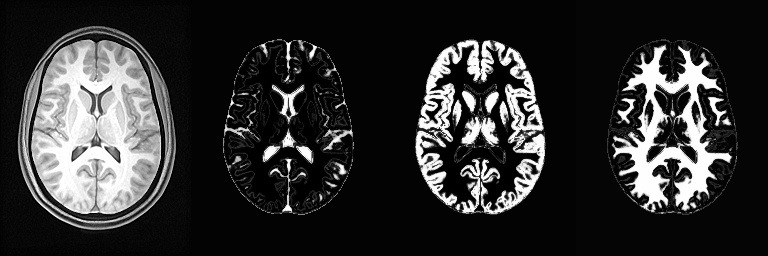
\includegraphics[width=0.9\textwidth]{templatefig.jpg} 
\itkcaption[Template Prior]{An example template.}
\vspace{-0.1in}
\label{fig:template}
\end{figure}

\section{Run a Cross-Sectional Study}
To run a pipedream study, your data needs to be organized as above and you need a template 
with all the necessary prior information available.  When all is ready, you will call:
\begin{verbatim}
    sh $PIPEDREAMDIR/pipedreamMapT1.sh pipedreamMapT1paramsUser.sh 
\end{verbatim}
where you likely have copied the ``base'' pipedreamMapT1paramsUser.sh
to your local directory and edited it for your data.  The output
directory structure and naming will mirror your input structure.  You
will get cortical thickness images, brain extraction, probability
maps, estimates of brain volume and---if enabled---a cortical
parcellation.

The key to the study is the file pipedreamMapT1paramsUser.sh.  
Within that file is a series of directory and then file variables that you need to define.  
We've tried to ``check'' your definitions for you and provide a warning that will help you 
find a mistake but this may not always work.  So, take care when making these definitions.

An important part of this step is how you distribute these processes.
We provide hooks for voxbo and for the SGE qsub.  There is also a
PIPEDREAMISTEST variable in the user configuration file that will set
``fast'' parameters to allow you to check your configuration before
running the full dataset.  Set variable GOTOVBQ=1, GOTOSGEQ=0 (for
voxbo) GOTOVBQ=0, GOTOSGEQ=1 (for sge) in pipedreamMapT1paramsUser.sh.  
If both are zero, you will run in serial mode. 

\section{Check Results}

Pipedream output is organized by subject and time point in a similar way to the input data, except that structural and DTI data are placed in the same directory. Within each time point output directory, there are the following files, prefixed with the subject ID and time point ID.

Images suffixed with ``norm.nii.gz" are normalized to standard space. If a mapping from the local template to standard space is provided, then all ``norm.nii.gz" are in standard space. Otherwise they are in the local template space. The images relating to DT processing are only produced if you have DT data for the subject and time point.

\begin{table}[htdp]
\caption{default}
\begin{center}
\begin{tabular}{| p{5cm} | p{10cm} |}
\hline
\textbf{Output} & \textbf{Description} \\ \hline
Affine.txt, InverseWarp.nii.gz, Warp.nii.gz & Warps from subject T1 to local template space. \\ \hline
brain.nii.gz & The brain-extracted and bias-corrected T1 image in subject space. \\ \hline
brainmask.nii.gz & The brain mask of the T1 image, used to compute brain.nii.gz. \\ \hline
brain\_prob\_[0,1,2].nii.gz & Segmentation probabilities of CSF (0), gray matter (1) and white matter in the T1 image. \\ \hline
deformed.nii.gz & Input head image deformed to the local template space. Useful for evaluating brain extraction and registration. \\ \hline
distcorr[Affine.txt, Warp.nii.gz, InverseWarp.nii.gz] & Distortion correction between T1 and DT space.\\ \hline
DTdeformed.nii.gz & DT image warped to the local template space \\ \hline
fa.nii.gz & Fractional anisotropy from DTI, in the subject space. \\ \hline
fadeformed.nii.gz & FA deformed into the local template space. \\ \hline
gmpnorm.nii.gz         & Normalized gray matter probability (brain\_prob\_1.nii.gz). \\ \hline
grid.nii.gz & Deformation grid showing the warp of the T1 image to template space. Used for evaluating registration. \\ \hline
head.nii.gz & Input T1 image. \\ \hline
kappa.nii.gz               & White matter curvature. \\ \hline
kappanorm.nii.gz   & kappa transformed to standard space. \\ \hline
logjacobian.nii.gz   & Log determinant of the Jacobian, in the local template space. \\ \hline
seg.nii.gz      & Three tissue segmentation of the T1 brain image.\\ \hline
thickness.nii.gz & Cortical thickness in the subject space. \\ \hline
thicknorm.nii.gz & Thickness warped to standard space. \\ \hline
\end{tabular}
\end{center}
\label{pipedreamMapT1out}
\caption{Output of pipedreamMapT1}
\end{table}%

If you have defined label images in the template space, there will be additional output containing the labels and probabilities in the subject space.

It's critical to evaluate the output data visually before doing statistics. The normalized images can be evaluated by extracting the same slice from all subjects, using ANTS:
\begin{verbatim}
    $ANTSPATH/StackSlices vol.nii.gz -1 -1 80  PipeDreamOutDir/*/*/*_thickness.nii.gz
\end{verbatim}
This will extract the 80th z-slice of every image and put it into a volume (vol.nii.gz) 
that you can scroll through.  You can call this on any image type.  If some specific dataset, e.g. subject00X, does not work, you 
may want to manually set the variable PIPEDREAMSUBJECTSLIST=subject00X and run a test 
on that subject alone, without sending to distributed computing, to see what is going on.  As above, if you 
set PIPEDREAMISTEST=1 you can get a fast test result for this subject.  

\section{Compute Statistics} 
If everything is good, you are ready to estimate group statistics.  We
prefer a {\bf R} statistical interface and can provide a script for
you.  However, you may run your favorite statistical package on the
output of pipedream.

\begin{comment}
\section{The PipeDream Preprocessing Pipeline} 
\subsection{Data Organization}
\subsection{T1 Pipeline} 
\subsection{DTI Pipeline}
\subsection{Quality Assurance}

\section{The PipeDream Cross-sectional Pipeline}

\subsection{The Importance of the Template}
\subsection{Customization}
\subsection{Required Software}

\section{The PipeDream Longitudinal Pipeline}

\section{A Working Example}
\subsection{The Template}
\subsection{The Data}
\subsection{The Results}
\subsection{The Longitudinal Results}
\end{comment}

\section{Annotated Bibliography}
The original statement of the symmetric normalization and template
construction methodology was given in \cite{Avants2004}.  A follow up
study that used landmark guidance to compare the chimpanzee cortex to
the human cortex was published here \cite{Avants2006} -- this study
used {\em in vivo} MRI and template-based normalization to confirm
volumetric numbers derived from an early 20th century post-mortem
study comparing one human and one chimp.  This conference article has
some additional detail and alternative updates to the methodology, in
particular application to shape-based interpolation
\cite{Avants2005b}.  Network based studies were performed here
\cite{duda08miccai,duda08cvpr}.  The main SyN paper is here
\cite{Avants2008}.  Applications to neurodegeneration are here
\cite{Avants2005,Avants2008a,Grossman2008,Avants2009,Das2009,Yushkevich2009,Massimo2009}.
Hippocampus focused work is here \cite{Pluta2009,Yushkevich2009}.  The
main evaluation papers include \cite{Avants2008} and \cite{Klein2009}
for the cortex and deep brain structures whereas \cite{Pluta2009}
evaluates the use of automated and semi-automated normalization for
high-throughput hippocampus morphometry.  An additional evaluation
paper is being developed.  


%%%%%%%%%%%%%%%%%%%%%%%%%%%%%%%%%%%%%%%%%
%
%  Insert the bibliography using BibTeX
%
%%%%%%%%%%%%%%%%%%%%%%%%%%%%%%%%%%%%%%%%%

\bibliographystyle{plain}
\bibliography{references,ants}


\end{document}

